\section{Uncertainty in PIV measurements}
\label{sec:piv_uncert}
 
There are a number of factors that contribute to uncertainty in PIV 
measurements. Both bias and precision errors can be estimated by considering 
detailed information about the optical geometry of the PIV setup. Monte-Carlo 
based error estimation techniques can be applied by creating artificially 
simulated images with randomly distributed particles \cite{adeyinka2005}. 
The distribution of these particles can be modeled using a Gaussian intensity  
profile by \cite{raffel1998} as described in Equation 
\ref{eq:piv_gaussian_uncertainty}.

\begin{equation}
	I(x,y) = I_0exp \left( \frac{-(x_{img} - x_p)^2 - (y_{img} - y_p)^2}
	{\frac{1}{8}d_\tau^2} \right)
	\label{eq:piv_gaussian_uncertainty}
\end{equation}

where $x_p$ and $y_p$ are the locations of the particle centroid, $d_\tau$ is 
the diameter of the particle, and $I_0$ is particle intensity. Particle 
intensity is directly related to the intensity of the light sheet, which is 
modeled as a Gaussian distribution \cite{PIVuncertAIAA}. This assumption allows 
us 
to express particle intensity as \ref{eq:particle_intensity_gaus}

\begin{equation}
	I_0(z_p) = (q)exp\left(- \frac{z_p^2}{\frac{1}{8}\Delta Z_L^2}\right)
	\label{eq:particle_intensity_gaus}
\end{equation}

where $z_p$ is the particles position within the thickness of the light sheet, 
$q$ is the particle light scattering efficiency, and $\Delta Z_L$ is the 
thickness of the light sheet.

These formula were used to generate artificial image pairs for a single camera. 
A sufficient number of particles were created with $x$, $y$ and $z$ coordinates 
to meet particle density parameters, these coordinates are then 
used to generate light intensities according to Equation 
\ref{eq:particle_intensity_gaus}, which populate the image plane of the first 
image $A$. Subsequently, a displacement image, $B$, was generated by shifting 
all the 
particles in a predetermined direction in three dimensional space. It is worth 
noting that for a single camera setup, particle movements in the $z$ direction 
do not produce pixel displacements, but simply determine the intensity of the 
light reflected from the particle. The known particle displacements can then be 
compared against outputs calculated with PIV capture and processing software.

To translate this concept to stereo PIV, an additional step was required. 
Instead of directly distributing particles with known coordinates onto the 
image 
plane of one camera, they were placed on a conceptual version of the 
interrogation plane. The coordinate transforms obtained from PIV calibration 
were used to map the displacements from the conceptual plane into the image 
plane of each camera. These coordinate transforms are unique to each camera, 
and depend upon the optical geometry of the PIV setup. Uncertainty is 
calculated using the recommended AIAA calibration procedure outlined in 
\cite{PIVuncertAIAA}. To determine the system bias, the mean difference between 
the velocity standard established by the Monte Carlo simulation and the 
velocity calculated by the PIV software are compared as follows

\begin{equation}
\overline{\Delta U} = \frac{1}{N} \left(\sum_{i=1}^N \Delta U_i \right),
\label{eq:Uerror}
\end{equation}

\begin{equation}
\overline{\Delta V} = \frac{1}{N} \left(\sum_{i=1}^N \Delta V_i \right),
\label{eq:Verror}
\end{equation}

\begin{equation}
\overline{\Delta W} = \frac{1}{N} \left(\sum_{i=1}^N \Delta W_i \right)
\label{eq:Werror}
\end{equation}

which is simply the average difference between the known velocity components 
and the measured velocity components $\Delta U$, $\Delta V$, and $\Delta W$, 
for a large number of simulations. This is referred to as the \textit{bias}, 
and the three bias components are denoted as

\begin{equation}
\beta_{U} = \overline{\Delta U},
\label{eq:Ubias}
\end{equation}
\begin{equation}
\beta_{V} = \overline{\Delta V},
\label{eq:Vbias}
\end{equation}
\begin{equation}
\beta_{W} = \overline{\Delta W},
\label{eq:Wbias}
\end{equation}

The measurement precision is reported as the root-mean-square of the  
standard deviation, calculated as in 
	
\begin{equation}
S_{\Delta U} = \sqrt{\frac{1}{N-1} \left(\sum_{i=1}^N (\Delta U_i - 
\overline{\Delta U})^2 \right)},
\label{eq:Usd}
\end{equation}

\begin{equation}
S_{\Delta V} = \sqrt{\frac{1}{N-1} \left(\sum_{i=1}^N (\Delta V_i - 
	\overline{\Delta V})^2 \right)},
\label{eq:Vsd}
\end{equation}

\begin{equation}
S_{\Delta W} = \sqrt{\frac{1}{N-1} \left(\sum_{i=1}^N (\Delta W_i - 
	\overline{\Delta W})^2 \right)},
\label{eq:Wsd}
\end{equation}

\noindent
resulting in precision calculations given by 
	
\begin{equation}
P_{\overline{U}} = \frac{2 S_{\Delta U}}{\sqrt{N}},
\label{eq:Uprec}
\end{equation}

\begin{equation}
P_{\overline{V}} = \frac{2 S_{\Delta V}}{\sqrt{N}},
\label{eq:Vprec}
\end{equation}

\begin{equation}
P_{\overline{W}} = \frac{2 S_{\Delta W}}{\sqrt{N}}
\label{eq:Wprec}
\end{equation}

Total uncertainty for each component at the 95\% confidence level was 
calculated by combining the bias and precision via to obtain

\begin{equation}
U_{\overline{\Delta U}} = \sqrt{\beta_{U}^2 + P_{\overline{U}}^2}
\label{eq:Uuncert}
\end{equation}
\begin{equation}
U_{\overline{\Delta V}} = \sqrt{\beta_{V}^2 + P_{\overline{V}}^2}
\label{eq:Vuncert}
\end{equation}
\begin{equation}
U_{\overline{\Delta W}} = \sqrt{\beta_{W}^2 + P_{\overline{W}}^2}
\label{eq:Wuncert}
\end{equation}


For these experiments, uncertainty analysis was conducted after the 
experimental data were taken. Vortices were characterized by velocities at key 
locations that allow each vortex to be described by one of the common vortex 
models. Characterization velocities of particular interest include the maximum 
tangential velocity about the vortex core, the distance of this maximal 
tangential velocity region from the core axis, which defined the core radius, 
and the typical 
axial velocity distribution near the free stream velocity. Understanding the 
uncertainty of these measurements required a Monte Carlo approach from 
synthetically created particle imagery as shown in Figures \ref{fig:la} and 
\ref{fig:lb}. Artificial pixel displacements were specified to approximate the 
typical displacement associated with the velocities of greatest interest. 

\begin{figure}[H]
	\centering
	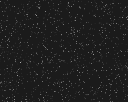
\includegraphics[width=4in]{figs/artificial_images/la}
	\caption{Left artificial image subset example, station 1, $t=0$.}
	\label{fig:la}
\end{figure}

\begin{figure}[H]
	\centering
	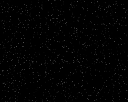
\includegraphics[width=4in]{figs/artificial_images/lb}
	\caption{Left artificial image subset example, station 1, $t=dt$.}
	\label{fig:lb}
\end{figure}

To add complexity, the time between frame captures, $dt$ was expected to have a 
significant impact on uncertainty. Since the range of velocities used in this 
study required the use of multiple values of $dt$, artificial images were 
generated for a scenario at each value of $dt$ with appropriate associated 
velocities. 
With the exception of measurements at station one, all tests were conducted 
with a $dt$ value of 25, or 40 $\mu s$. At station one $dt$ values of 35 $\mu 
s$ were also used. During the experimentation period, great difficulty 
was encountered in tuning PIV parameters to achieve well-resolved vector fields 
at station one. The uncertainty analysis demonstrated that the actual geometry 
of the viewing angles was also unfavorable at this station, and the quality of 
measurements taken this far upstream was poor. Hence, that data was entirely 
disregarded.

Creation of these artificial images by Monte Carlo was performed with custom 
software written in Python\texttrademark. This software parses the calibration 
files output 
from INSIGHT software and constructs the set of equations needed for all 
coordinate transformations. In order to simulate as accurately as possible, 
artificial images were generated at the full resolution of the specific PIV 
cameras, (1280 x 1024). Particles were only generated randomly at coordinates 
that were within the field of view of both cameras, to eliminate wasted 
computation time generating particles which would not aid in the production of 
a three-dimensional vector. An excess of 100,000 particles were simulated for 
each image set in order to ensure that the particle density was sufficient to 
resolve a vector in the majority of sectors, and to approximate the 
experimental seed density as closely as possible. The most accurate way to 
ensure that the intensities of each particle was represented accurately was to 
evaluate the intensity for every particle at every point in the full image 
space of 1280 x 1024 pixels, and then add them together. Since this produces a 
three-dimensional space in excess 
of a five billion values for a set of $La, Lb, Ra$ and $Rb$ images, computation 
time for uncertainty images was a limiting factor. At a minimum, one set of 
uncertainty images for each combination of viewing geometry and time step $dt$ 
was required. Therefore, simulated velocity values were chosen for each of the 
14 cases to approximate the velocities of greatest interest. 

Tables \ref{table:experiment_results_1} through 
\ref{table:experiment_results_7} show a summary of results from each of the 70 
tests conducted, including the maximum 
observed azimuthal velocity, the average measured axial velocity, and the low 
axial velocity at the vortex core. At the three furthest positions downstream 
where the vortex appears to have stabilized, the typical value of maximum 
tangential velocity, $\overline{v_{\theta, max}$ in component notation, ranges 
from 6.0 to 7.9 $m/s$ for each run with a $dt$ of $25 \mu s$. This tangential 
velocity could align with the $X$ or $Y$-axis, and 
it was desirable to simulate displacements in both directions at once to limit 
the number of Monte Carlo simulations to be performed, so simulated velocities
$\overline{u}_{sim}$ and $\overline{v}_{sim}$
of $4.9 m/s$ was employed so that the in-plane magnitude would be equal 
to the the middle of this range. Likewise, a simulated $\overline{u}_{sim}$ and 
$\overline{v}_{sim}$  velocity of 
$3.3 m/s$ was used to create synthetic images for testing experiments with a 
$dt$ of $40 \mu s$. In the axial direction, $Z$ , mean values of $19 m/s$ and 
$29 
m/s$ were used for the high and low velocity experiments respectively. These 
conditions are summarized in Table \ref{table:uncertainty_sim_table}.

\begin{table}[H]
\begin{center}
\begin{tabular}{|ccccc|}
	\hline
	Applies to & $dt$ & $\overline{u}_{sim}$ & $\overline{v}_{sim}$ & $\overline{w}_{sim}$\\
	  & $\mu s$ & $m/s$ & $m/s$ & $m/s$\\
	\hline
	Experiments where $V_{fs} < 24 m/s$ & 40 & 3.3 & 3.3 & 16\\
	Experiments where $V_{fs} > 24 m/s$ & 25 & 4.9 & 4.9 & 24\\
	\hline
\end{tabular}
\caption{Velocity conditions of Monte Carlo image generation for uncertainty analysis.}
\label{table:uncertainty_sim_table}
\end{center}
\end{table}


Even though many samples were taken at every vector location, the uncertainty 
in each individual measurement was of great importance for studying the 
unsteady component of the velocity, and thus turbulent phenomena. Uncertainty 
in the fluctuating component were best represented by using an $N$-value of one 
in precision Equations \ref{eq:Uprec} through \ref{eq:Wprec}. 
Uncertainty in the stable component was lower, since this measurement is a 
result of averaging many measurements, and was calculated by using an $N$-value 
of 200 in the precision Equations \ref{eq:Uprec} through \ref{eq:Wprec}.


\subsection{Uncertainty Analysis Results}
The Monte Carlo analysis was performed for each station employing two 
scenarios. Uncertainty in the measurements for $u, v$ and $w$ 
components are tabulated in Tables \ref{table:uncertainties_u} through 
\ref{table:uncertainties_w}. For the $u$ velocity components in the $X$ 
direction, bias is reported as $\beta_u$, 
precisions are reported for both single-sample measurements and with 
measurements comprised of 200 averages by $P_{u^\prime}$ and $P_{\bar{u}}$ 
respectively. Total uncertainties are reported as $U_{u^\prime}$ and 
$U_{\bar{u}}$. 

\renewcommand\baselinestretch{1.3}\selectfont
\begin{table}[H]
\begin{center}
\begin{tabular}{|ccccccccccc|}
	\hline
	Station & $dt$ & $u_{sim}$ & $v_{sim}$ & $w_{sim}$ & $\bar{u}$ & $\beta_u$ & $P_{u^{\prime}}$ & $P_{\bar{u}}$ & $U_{u^{\prime}}$ & $U_{\bar{u}}$\\
	\hline
	1 & 25 & 6.15 & 6.15 & 24.0 & 6.756 & 0.606 & 1.883 & 0.133 & 1.978 & 0.620\\
	1 & 40 & 5.6 & 5.6 & 16.0 & 5.759 & 0.159 & 0.717 & 0.051 & 0.735 & 0.167\\
	2 & 25 & 6.15 & 6.15 & 24.0 & 6.247 & 0.097 & 2.480 & 0.175 & 2.482 & 0.201\\
	2 & 40 & 5.6 & 5.6 & 16.0 & 5.557 & -0.043 & 1.300 & 0.092 & 1.301 & 0.101\\
	3 & 25 & 6.15 & 6.15 & 24.0 & 5.492 & -0.658 & 1.282 & 0.091 & 1.442 & 0.665\\
	3 & 40 & 5.6 & 5.6 & 16.0 & 5.588 & -0.012 & 1.354 & 0.096 & 1.354 & 0.097\\
	4 & 25 & 6.15 & 6.15 & 24.0 & 5.610 & -0.540 & 0.975 & 0.069 & 1.114 & 0.544\\
	4 & 40 & 5.6 & 5.6 & 16.0 & 5.696 & 0.096 & 0.844 & 0.060 & 0.849 & 0.113\\
	5 & 25 & 6.15 & 6.15 & 24.0 & 6.579 & 0.429 & 1.608 & 0.114 & 1.664 & 0.444\\
	5 & 40 & 5.6 & 5.6 & 16.0 & 5.917 & 0.317 & 0.667 & 0.047 & 0.738 & 0.321\\
	6 & 25 & 6.15 & 6.15 & 24.0 & 7.366 & 1.216 & 1.463 & 0.103 & 1.902 & 1.220\\
	6 & 40 & 5.6 & 5.6 & 16.0 & 5.841 & 0.241 & 0.595 & 0.042 & 0.642 & 0.245\\
	7 & 25 & 6.15 & 6.15 & 24.0 & 6.972 & 0.822 & 1.885 & 0.133 & 2.056 & 0.832\\
	7 & 40 & 5.6 & 5.6 & 16.0 & 5.688 & 0.088 & 1.014 & 0.072 & 1.018 & 0.114\\
	\hline
\end{tabular}
\caption{Uncertainty in $X$ direction velocity measurements. Unlabelled units are $m/s$.}
\label{table:uncertainties_u}
\end{center}
\end{table}
\renewcommand\baselinestretch{2}\selectfont

\renewcommand\baselinestretch{1.3}\selectfont
\begin{table}[H]
\begin{center}
\begin{tabular}{|ccccccccccc|}
	\hline
	Station & $dt$ & $u_{sim}$ & $v_{sim}$ & $w_{sim}$ & $\bar{v}$ & $\beta_v$ & $P_{v^{\prime}}$ & $P_{\bar{v}}$ & $U_{v^{\prime}}$ & $U_{\bar{v}}$\\
	\hline
	1 & 25 & 6.15 & 6.15 & 24.0 & 5.155 & -0.995 & 0.717 & 0.051 & 1.226 & 0.996\\
	1 & 40 & 5.6 & 5.6 & 16.0 & 4.159 & -1.441 & 0.444 & 0.031 & 1.508 & 1.441\\
	2 & 25 & 6.15 & 6.15 & 24.0 & 5.597 & -0.553 & 0.615 & 0.044 & 0.827 & 0.554\\
	2 & 40 & 5.6 & 5.6 & 16.0 & 4.805 & -0.795 & 0.744 & 0.053 & 1.089 & 0.797\\
	3 & 25 & 6.15 & 6.15 & 24.0 & 5.530 & -0.620 & 0.545 & 0.039 & 0.825 & 0.621\\
	3 & 40 & 5.6 & 5.6 & 16.0 & 4.790 & -0.810 & 0.538 & 0.038 & 0.973 & 0.811\\
	4 & 25 & 6.15 & 6.15 & 24.0 & 5.585 & -0.565 & 0.588 & 0.042 & 0.815 & 0.567\\
	4 & 40 & 5.6 & 5.6 & 16.0 & 4.902 & -0.698 & 0.537 & 0.038 & 0.881 & 0.699\\
	5 & 25 & 6.15 & 6.15 & 24.0 & 5.729 & -0.421 & 0.623 & 0.044 & 0.752 & 0.424\\
	5 & 40 & 5.6 & 5.6 & 16.0 & 5.153 & -0.447 & 0.510 & 0.036 & 0.679 & 0.449\\
	6 & 25 & 6.15 & 6.15 & 24.0 & 5.832 & -0.318 & 0.744 & 0.053 & 0.809 & 0.322\\
	6 & 40 & 5.6 & 5.6 & 16.0 & 5.301 & -0.299 & 0.534 & 0.038 & 0.612 & 0.301\\
	7 & 25 & 6.15 & 6.15 & 24.0 & 6.060 & -0.090 & 0.780 & 0.055 & 0.785 & 0.106\\
	7 & 40 & 5.6 & 5.6 & 16.0 & 5.579 & -0.021 & 0.633 & 0.045 & 0.633 & 0.050\\
	\hline
\end{tabular}
\caption{Uncertainty in $Y$ direction velocity measurements. Unlabelled units are $m/s$.}
\label{table:uncertainties_v}
\end{center}
\end{table}
\renewcommand\baselinestretch{2}\selectfont

\begin{table}[H]
\begin{center}
\begin{tabular}{|ccccccccccc|}
	\hline
	Station & $dt$ & $u_{sim}$ & $v_{sim}$ & $w_{sim}$ & $\bar{w}$ & $\beta_w$ & $P_{w^{\prime}}$ & $P_{\bar{w}}$ & $U_{w^{\prime}}$ & $U_{\bar{w}}$\\
	\hline
	1 & 25 & 4.900 & 4.900 & 29.000 & 18.598 & -10.402 & 0.770 & 0.054 & 10.431 & 10.402\\
	1 & 40 & 3.300 & 3.300 & 19.000 & 11.834 & -7.166 & 0.372 & 0.026 & 7.176 & 7.166\\
	2 & 25 & 4.900 & 4.900 & 29.000 & 19.882 & -9.118 & 0.663 & 0.047 & 9.142 & 9.118\\
	2 & 40 & 3.300 & 3.300 & 19.000 & 12.993 & -6.007 & 0.684 & 0.048 & 6.045 & 6.007\\
	3 & 25 & 4.900 & 4.900 & 29.000 & 22.271 & -6.729 & 1.752 & 0.124 & 6.954 & 6.730\\
	3 & 40 & 3.300 & 3.300 & 19.000 & 15.310 & -3.690 & 0.928 & 0.066 & 3.805 & 3.691\\
	4 & 25 & 4.900 & 4.900 & 29.000 & 25.811 & -3.189 & 0.948 & 0.067 & 3.327 & 3.189\\
	4 & 40 & 3.300 & 3.300 & 19.000 & 16.657 & -2.343 & 0.358 & 0.025 & 2.371 & 2.344\\
	5 & 25 & 4.900 & 4.900 & 29.000 & 26.704 & -2.296 & 0.562 & 0.040 & 2.364 & 2.297\\
	5 & 40 & 3.300 & 3.300 & 19.000 & 17.006 & -1.994 & 0.297 & 0.021 & 2.016 & 1.994\\
	6 & 25 & 4.900 & 4.900 & 29.000 & 27.204 & -1.796 & 0.503 & 0.036 & 1.865 & 1.796\\
	6 & 40 & 3.300 & 3.300 & 19.000 & 17.398 & -1.602 & 0.502 & 0.036 & 1.679 & 1.602\\
	7 & 25 & 4.900 & 4.900 & 29.000 & 28.094 & -0.906 & 0.953 & 0.067 & 1.314 & 0.908\\
	7 & 40 & 3.300 & 3.300 & 19.000 & 18.626 & -0.374 & 0.931 & 0.066 & 1.003 & 0.380\\
	\hline
\end{tabular}
\caption{Uncertainty in $Z$ direction velocity measurements. Unlabelled units are $m/s$.}
\label{table:uncertainties_w}
\end{center}
\end{table}


The results of the Monte Carlo analysis held some surprises. Uncertainties in 
the $X$ and $Y$ direction were comparable in some cases, while in others $Y$ 
uncertainties were half as high as those in $X$. At all velocities, poor 
precision in the individual measurements was the primary driver of total 
uncertainty, while high bias was the driver for uncertainties in the 
measurements comprised of time averages of 200 samples. Spectral analysis of 
the turbulence over the observation time is subject to the very high 
uncertainties associated with that of individual measurements. Time averaged 
velocities, and the derived Reynolds stresses are best characterized by the 
better precision offered by many samples. While 200 is nominally used as $N$, 
each grid point may have between 20 and 200 valid vectors making up the set, so 
some areas where vectors were less frequently resolved successfully may be 
characterized with greater uncertainty.

In the axial or $Z$-direction, the PIV was found to exhibit an extreme bias 
toward underestimating velocities based on the Monte Carlo simulation. This 
bias starts at over 30\% at the closest station, and diminishes systematically 
with downstream position and decreasing velocity. However, experimental data 
showed that the average axial velocity was consistently a few percent above 
free stream velocity measured in the wind tunnel using dynamic pressure 
instrumentation, as expected, as shown in Tables 
\ref{table:experiment_results_1} through \ref{table:experiment_results_7}. 
Therefore, uncertainties in the $Z$ direction were overestimated by the 
technique. The mean component of the Reynolds decomposition components are 
strongly influenced by a high bias, but the fluctuating components are entirely 
sensitive to precision. The Reynolds stress and turbulence values which are of 
great importance in this study included contributions of velocity fluctuations 
in the axial direction, which are not impacted by any bias that does exist. 
Experimental data were examined for possible misrepresentation of measurement 
uncertainty in the $X$ and $Y$ direction, but no statistically meaningful 
discrepancies were found. Histograms the distribution of measurements for each 
of the 14 cases were included in Appendix \ref{appendix:uncertainty_histograms}.


\subsection{Bias from Uneven sampling}

Every grid location with at least 20 successfully resolved vectors was 
subject to a Reynolds decomposition into average and fluctuating components. 
With 200 total samples taken for each test, the results are actually made up of 
many grid points with between 20 and 200 samples. Uncertainty is related to the 
number of samples making up a measurement, but visualizing the potential 
impacts of uncertainty as it varies in two and three dimensional space is 
challenging. Furthermore, the likelihood of successfully resolving a vector is 
dependent upon aspects of the interaction between tracer particles and the 
fluid flow. A very clear interdependence between areas of high turbulence, and 
the number of successful vector calculations was observed as shown in Figures 
\ref{fig:run_55_num_contour} and \ref{fig:run_55_ctke_contour}. 

\begin{figure}[H]
\centering
\includegraphics[width=4.25in]{figs/run_55/run_55_num_contour}
\caption{Contour plot of $N$ at $z/c$=9.50, $V_{free}$=23.33, station 6.}
\label{fig:run_55_num_contour}
\end{figure}



\begin{figure}[H]
\centering
\includegraphics[width=4.25in]{figs/run_55/run_55_ctke_contour}
\caption{Contour plot of $k$ at $z/c$=9.50, $V_{free}$=23.33, station 6.}
\label{fig:run_55_ctke_contour}
\end{figure}




It was assumed that, as long as the number of samples making up any given 
measurement remains above the threshold of 20, every vector in the field is 
accurately represented. A sampling technique could be employed by 
which a random selection of 20 different values is used at every location, to 
result in a more statistically homogeneous vector field. However, 
the uncertainty in a PIV measurement also depends significantly on the 
magnitude of the velocity measured, so the benefit of such a sampling scheme is 
contestable.